\documentclass{article}
\usepackage[T1]{fontenc}
\usepackage{lmodern}
\usepackage{graphicx}
\usepackage{amsmath,amssymb}
\usepackage[a4paper,margin=2cm]{geometry}
\usepackage[absolute,overlay]{textpos}
\setlength{\TPHorizModule}{1mm}
\setlength{\TPVertModule}{1mm}
\usepackage[indonesian]{babel}
\usepackage{hyperref}
\setlength{\emergencystretch}{2em}
% unit: Halaman 46

\begin{document}

% === Halaman 46 (python/native) ===

46

• PRGA membangkitkan kunci-alir (keystream) dengan cara mengambil nilai S[i] dan 

S[j], mempertukarkannya, lalu menjumlahkan keduanya dalam modulus 256. 

• Kunci alir tersebut kemudian di-XOR-kan dengan sebuah karakter plainteks.


 i  0

 j  0

 for idx  0 to Length(P) – 1 do

     i  (i + 1) mod 256

     j  (j + S[i]) mod 256


 swap(S[i], S[j])   \{* Pertukarkan nilai S[i] dan S[j] *\}


 t  (S[i] + S[j]) mod 256


 u  S[t]         (* keystream *)


 c  u  P[idx]   \{ enkripsi \}

 end

Pseudo-random generation algorithm (PRGA)

% deskripsi: gambar native xref 216
\noindent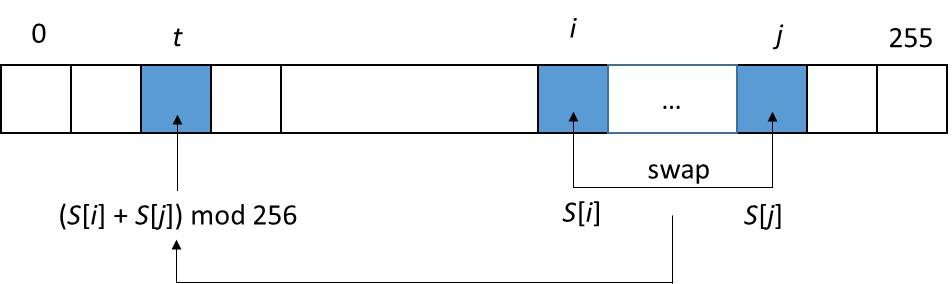
\includegraphics[width=0.85\textwidth]{../../images/python/page_046_img_01.jpeg}

\end{document}
